\documentclass[bibliography=totoc]{article}
\usepackage[T1]{fontenc}
\usepackage[utf8]{inputenc}
\usepackage[ngerman, english]{babel}

\usepackage{hyperref}
\usepackage{tikz}
\usepackage{tikz-qtree}
\usepackage{tikz-qtree-compat}
\usepackage{graphicx} 
\usepackage{float}

\title{University of Stuttgart \vspace{1em}\\Text Technology Project Report}
\author{Instructor: Andre Blessing\\Students: Brandon Sorensen, King DeLaney, \\Haywood Shannon, Johannes Krämer}
\date{2019}

\begin{document}
\maketitle


\section{Elasticsearch Project}
Why did we choose Elasticsearch? "You know, for Search."
\\
\\
But seriously, Elasticsearch is a state of the art tool. It is used by 
research and industry extensively. This should be enough reason. Hearing the buzzword "Elasticsearch" 
certainly motivated us in this direction. But the real fascination came by watching
introductory Youtube videos about Elasticsearch. Most people were so positively 
excited while talking about it that we basically were conviced about 
the power of Elasticsearch before even trying it out.
\\  
\\
Our project approach was a heterogeneous one. Our goal was to explore, play around, learn about the full power of 
Elasticsearch without beeing bound to a specific downstream task.
As a result we have used different datasets to illustrate different capabilities of the technology:
the ufo dataset, the beer dataset and the political dataset.

\section{The ELK Stack}
The ELK Stack stands for Elasticsearch, Logstash, and Kibana.
These three technologies are often referred to when talking about Elasticsearch
on it's own. The reason is because together they form a pipeline where
Elasticsearch as a database is the core technology.
\\
From a dataflow point of view, Logstash is the first technology. It servers
as a preprocessing tool which brings the data in the right shape. The second 
tool is Elasticsearch which stores and index the data. The third tool is 
Kibana, which provides a Graphical User Interface (GUI) to Elasticsearch's data 
and is reponsible for visualizing the data. 
\\
The ELK Stack, is available for personal usage for free. But it can also be 
employed professionaly by either using it as Software as a Service (SaaS) in the Cloud,
or by integrating it in the company server centers. With the last two approaches 
the above mentioned technologies are perfectly scalable to basically any size of data/storage,
computing power.

\subsection{Logstash}
\begin{figure}
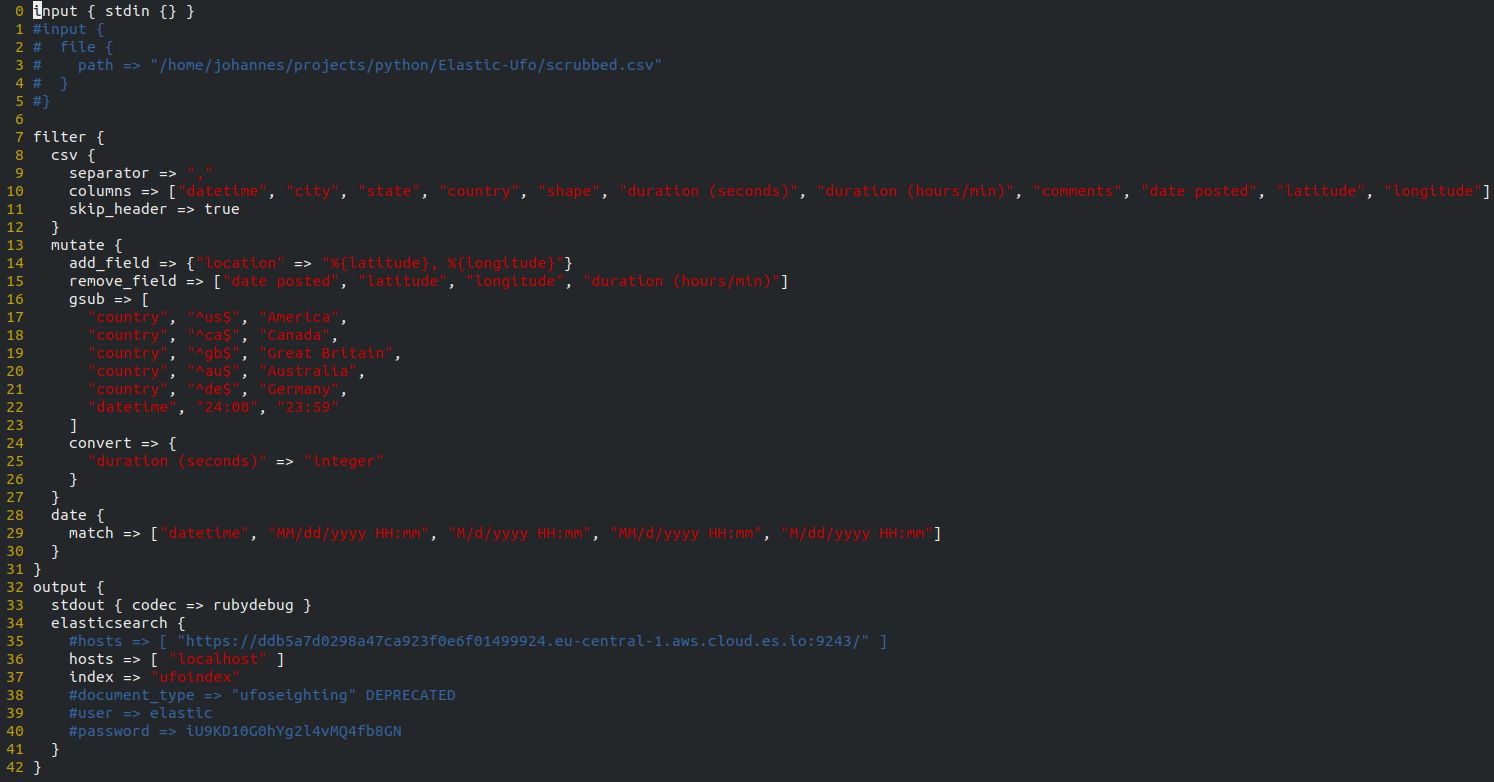
\includegraphics[height=0.5\textwidth]{logstash_config.png}
\caption{\label{logstash_config_file}
The Logstash configuration file which was used to preprocess the Ufo dataset.}
\end{figure}

As already mentioned Logstash can be seen as a preprocessing tool.
It prepares the data and sends the transformed data to the specified 
Elasticsearch instance.
It is able to recieve data from all kinds of sources in all kinds of formats like from Databases, HTTP-Streams, 
CSV-files, JSON-files, Logfiles etc.
\\
With the help of filters the data is parsed and transformed into a
desired format. That way it is possible to achieve more structure, consistancy,
readability etc.
\\
In the next paragraph the configuration file which was used for the
Ufo-sighting project will be explained (see Figure \ref{logstash_config_file}).
\\
The Ufo-sightings are stored in a csv file. Hence the configuration file 
contains definitions specific for a csv file.
\\
In line 0-5 the input is defined (the csv file). Once dynamically read 
from the standart input \footnote{means the path to the file needs to be passed as an argument when running logstash} (stdin),
and once with a hardcoded path to the csv file.
\\
From line 7-31 different filters are defined which deal with the content 
of the csv file:
\\
The csv filter (line 8-12) specifies the structure of the original csv file.
In this case the csv file is comma seperated (could be tab seperated aswell),
has the following columns (see image) and the header is skipped because
it is not part of the actual data.
\\
The mutate filters (line 13-27) actually applied some changes to the data:
In line 14 we a new field \textit{location} is constructed out of the 
existing \textit{latitude} and \textit{longitude} fields. The reason for 
that is, that in order to represent geo-coordinates Elasticsearch requires geographical data to be stored as a tuple
in one field instead of beeing stored in seperate fields.
\\
On line 15 a couple of fields are removed, which where decided to be not relevant
for the data analysis anymore. For example geographical information is now 
stored in the \textit{location} field, hence the original \textit{lalitude}- and \textit{longitude}-fields
are not needed anymore.
\\
The \textit{gsup} mutation (line 16-23) is a regular expression based string subsitution.
The first column defines the source field, the second column defines the regular expression
and the third field is the replacement string.
\\
In this case the language codes are transformed into the original country names
just for the sake of readability.
\\
The last subsitution is a little hack to deal with a specificity of the Ufo-dataset.
In the Ufo-dataset midnight was encoded as 24:00. But Elasticsearch's time format goes from
00:00:00-23:59:59. Although it is more common to represent midnight as 00:00, sometimes
24:00 is used to represent the end of the day and 00:00 the beginning of the day.
Since the original midnight encoding was 24:00 (end of day) it was decided to 
remove one minute instead of adding one, such that the time still represents the end 
of a day instead of the beginning of the next day.
\\
The date filter (line 28-30) deals with different date representations.
Elasticsearch requires a consistent date-time representation to be automatically
recognized as such. Therefore all possible date combinations\footnote{A day represented with one digit. A day represented as two digits. A month represented as one digit. A month represented as two digits.} must be 
given to the date filter.
The first entry is the column name of the date field followed by the 
different possible combinations of date representation.
\\
\\
From line 32-42 the output is defined. This means where the transformed data is 
sent to:
In line 33 debugging information is sent to the standart output (stdout) - e.g. the console.
From line 34-41 the Elasticsearch target instance is defined together with the 
index the data should be stored at. In this case (line 36) Elasticsearch
runs locally (localhost) and the index (line 37) is called \textit{ufoindex}.
\\
As mentioned earlier Elasticsearch can be used as a service in the cloud. In line 
35 a Elasticsearch target instance can be seen which was hosted on Amazons AWS Cloud-system\footnote{A free trial was used in order to have all the material for the presentation ready in one place. The trial (and hence the url) is not active anymore.}.

\subsection{Elasticsearch}
As already mentioned Elasticsearch is a database and a search engine.
The following query and search examples were made with the beer dataset.

\subsubsection{Query Language}
\begin{figure}
   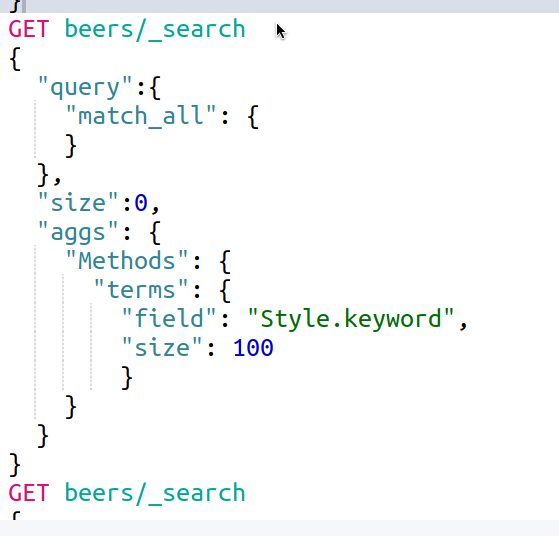
\includegraphics[height=0.7\textwidth]{beer_query_language.png}
   \caption{\label{beer_query_language}Example for the Elasticsearch Query Language} 
\end{figure}
Elastic search queries use a structure similar to JSON (see Figure \ref{beer_query_language}).
All features of the query are nested within within the “query” field, 
and sub-fields such as “match”, “bool”, and “wildcard” are 
there to match the needs of the user. 
Within the query, filters, modifications, and precision adjustments 
can also be implemented.
Attributes of the query such as “size” are beneath and not nested 
directly in the original query. The size field will control the 
number of results of the query or “buckets” during aggregation. 
Additionally, actions such as aggregations are also outside and below 
the query. Additional aggregations, can also be added to the end 
or within other aggregations.

\subsubsection{Mapping}
\begin{figure}
    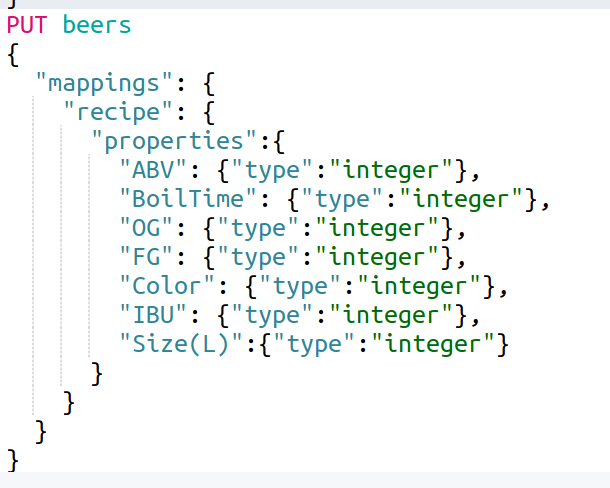
\includegraphics[height=0.7\textwidth]{beer_mapping.png}
    \caption{\label{beer_mapping}Example for a Mapping} 
 \end{figure}
Data being stored in Elasticsearch is a stringified JSON format. 
Mappings (see Figure \ref{beer_mapping}) are needed to provide the structure to values that are to 
be extracted and evaluated in methods other than those of plain text. 
JSON Mappings allow for basic types beyond strings such as integers, dates, 
Boolean values, and range data.  
There are also more complex types, like arrays and dictionaries 
(or other JSON structured data), 
and additionally, there more specific data types such as Geo-point and 
IP data types.
For values that are integers or a more complex data type  and 
would like to be use for searches, aggregations within a range, 
plotted over a geographical map a mapping of the index must be 
used to create the index.
In this mapping, the index “beers” has seven fields where the values 
will be type “integer” the remaining as well as any additional fields will 
be recognized as type “string”.

\subsubsection{Basic Search}
\begin{figure}
    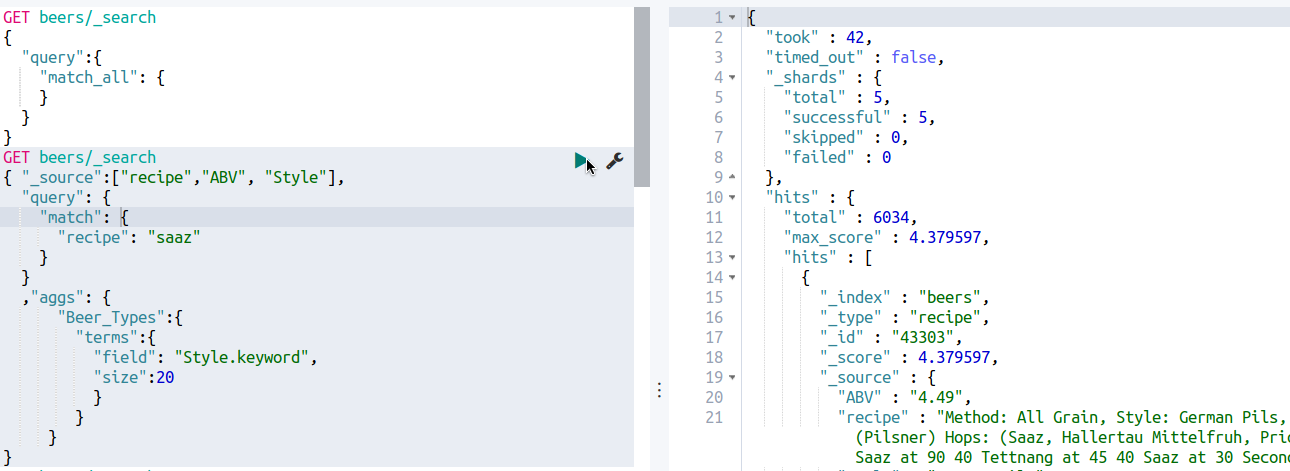
\includegraphics[height=0.4\textwidth]{basic_search.png}
    \caption{\label{beer_basic_search}Example for a basic search usecase} 
 \end{figure}
 The basic search allows to match a value to specific fields or just searched over 
 the whole of each document in the index. 
 In the queries (see Figure \ref{beer_basic_search}), there is a basic search for all items in the 
 index and a query for the string value “saaz” from the specific field 
 “recipe” . The second search also has limit to which fields of 
the document within the index will be presented within the query 
results. By selecting “source”, we specified the fields “recipe”, 
 “ABV”, and “Style” to be present in the query results.  

 \subsubsection{Aggregations}
 \begin{figure}
    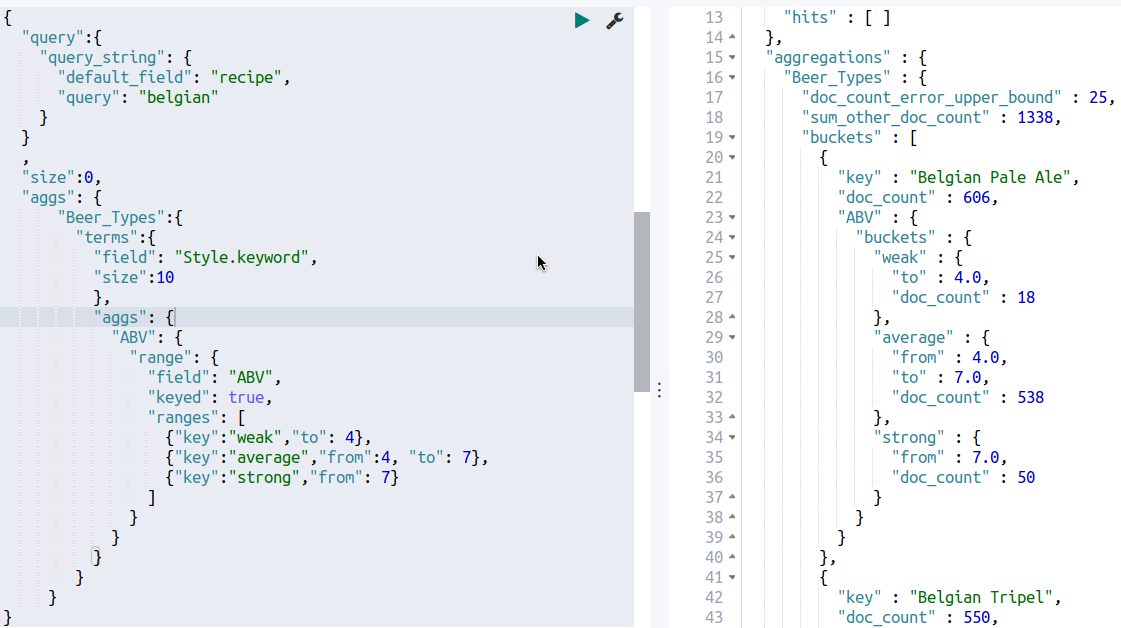
\includegraphics[height=0.6\textwidth]{beer_aggregations.png}
    \caption{\label{beer_aggregations}Example for aggregations} 
 \end{figure}
 Elasticsearch allows for quick aggregations from a variety of different means. 
 Aggregations can made on unique field values or ranges as well as a filter 
 value that can be applied to a given aggregation. 
 Limits can also be set with the “size” field within the query to limit or 
 expand the number of query and/or aggregation results.
 In this query (see Figure \ref{beer_aggregations}), we have utilized the unique values of within the field 
 “Style” to first aggregate the result documents of a string-query 
 for the value “belgian” . The number of styles was limited to ten 
 style “buckets”, and within those buckets, we were once again able 
 to aggregate them according the range value of “ABV”. 
 We have only three ranges here, but the limit is at least one, 
 with an indetermined upper-bound limit. 

\subsubsection{Weighted and Wildcard Queries}
\begin{figure}
    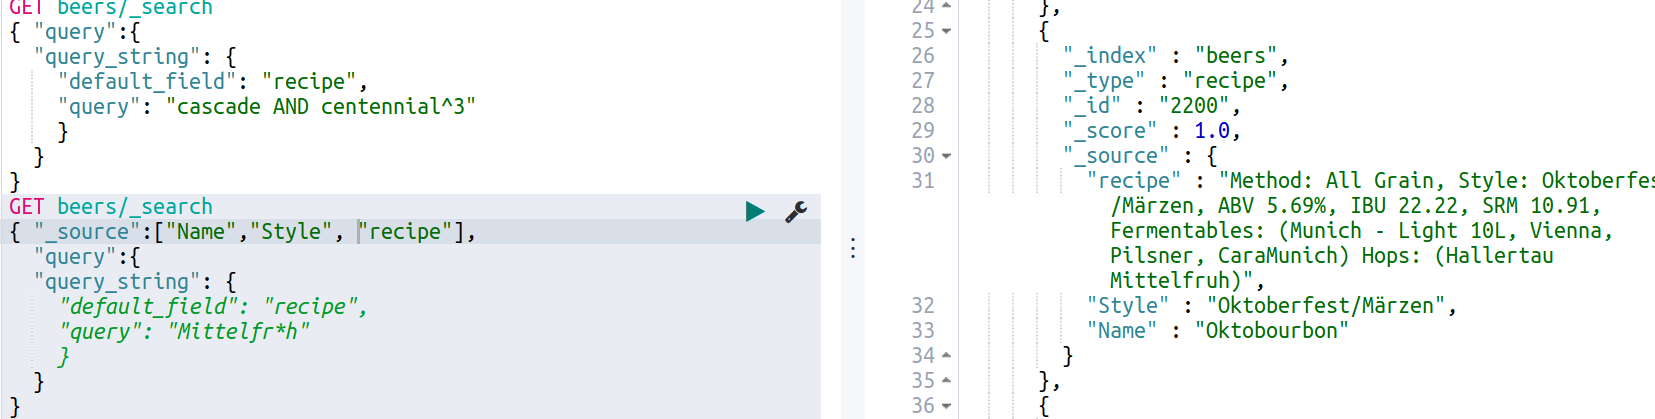
\includegraphics[height=0.3\textwidth]{beer_wildcard.png}
    \caption{\label{beer_wildcard}Example for weighted and wildcard queries} 
 \end{figure}
Elasticsearch allows for weighting or boosting the significance of 
a query term. In the a query, the “\^{}” symbol is used to begin the 
boosting of a specific term. This boosting can occur over many 
values and each will adjust the weighted ranking of the result documents. In this instance, we made the value of “centennial” three times more significant in the ranked results than the value “cascade”. 
Wildcard queries are also easily performed in Elasticsearch. 
The “*” character is used for wildcard queries. In the query (see Figure \ref{beer_wildcard}), 
we used a wildcard for the value “Mittelfrüh”. 
Terms with characters that are less common, in this case the “u” with 
an umlaut, might return results with correct and incorrect spellings 
of the term. 
 
\subsubsection{Proximity and Precision}
\begin{figure}
    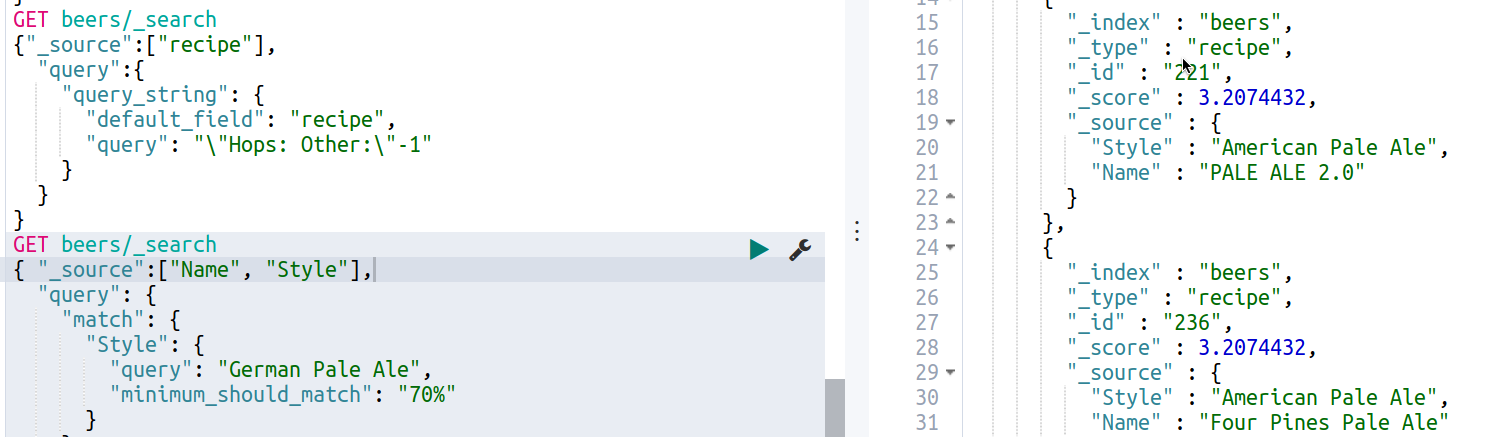
\includegraphics[height=0.3\textwidth]{beer_proximity.png}
    \caption{\label{beer_proximity}Example for proximity and precision} 
 \end{figure}
 A feature of Elasticsearch text search is proximity searches. 
 The use of boundary “\textbackslash” and quotes can define the values and a 
 number outside will define the proximity space between the two 
 terms. In the query (see Figure \ref{beer_proximity}), it queries for “Hops:” and “Other:” 
 separated by no more than one additional term between. 
 Additionally, precision within the searches can be improved by 
 targeting a minimum match. Using the field “minimum-should-match”, 
 a string percentage value is given by which Elasticsearch tries to 
 match to as a minimum. The 
 percentage may be decreased to the nearest evenly distributed percentage 
 based on the length of the query. 
 In our query “German Pale Ale”, our likely distribution is 
 that each word constitutes 33.33\% of the query. 
 If we match to “70”, it will try to match at least 66.67\%. 
 Within the results, “Pale Ale” is most likely to occur and returns 
 many results with style “American Pale Ale”.

 \subsubsection{Beer Dataset}
 \begin{figure}
    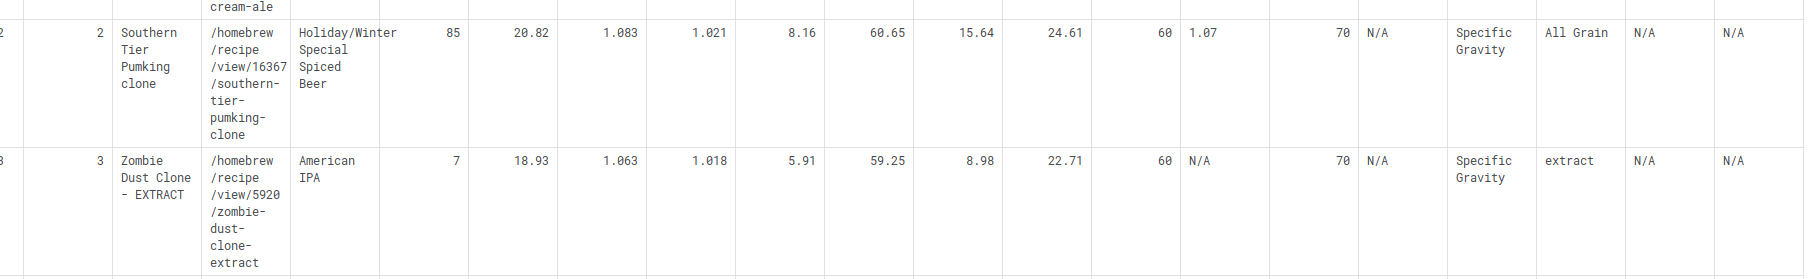
\includegraphics[height=0.2\textwidth]{beer_dataset.png}
    \caption{\label{beer_dataset}An excerpt of the beer dataset} 
 \end{figure}
 The Brewer’s Friend Beer recipe dataset (see Figure \ref{beer_dataset}) that was selected started 
 from Kaggle.com. It contained several fields already, 
 including several aspects of a beers color, alcohol content, 
 style, etc. The dataset was, however, lacking in areas 
 involving methodology and ingredients. To make a more 
 comprehensive and interesting dateset, more data needed to be 
 gathered. For each entry, there was a link the recipe page where 
 more information about the recipe could be ascertained. 
 Extracting the data for each recipe would be the most effective 
 way to compile more data into this data set.

 \subsubsection{Crawler}
 \begin{figure}
    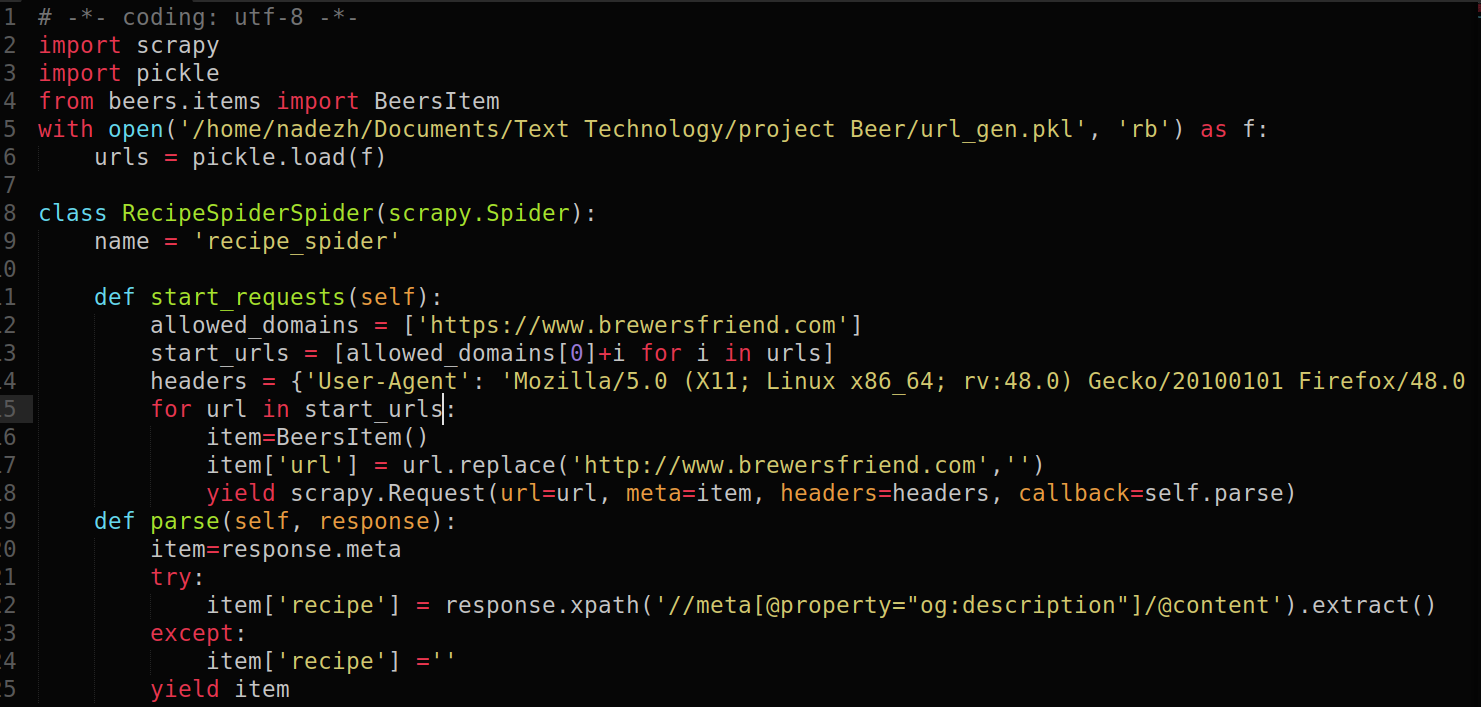
\includegraphics[height=0.5\textwidth]{beer_crawler.png}
    \caption{\label{beer_crawler}Scrapy Spider Code} 
 \end{figure}
 For this particular website, the recipe data was in several tables 
 throughout the page. The corresponding data was also located 
 in meta tags within the Html. This spider was constructed via 
 Scrapy (see Figure \ref{beer_crawler}). It sifted through the list of urls created from the 
 Brewer’s friend website and the recipe extension from the 
 dataset. It extracted the attribute data from the meta tags. 
 This data contained some of the data found in the original data 
 set as well as various types of ingredients in up to four different 
 categories and notes that the author felt necessary. 
 All data was extracted to CSV files in smaller batches as the 
 process of scraping 73,000 recipes took over 70 hours.   

 \subsubsection{Extraction}
 \begin{figure}
    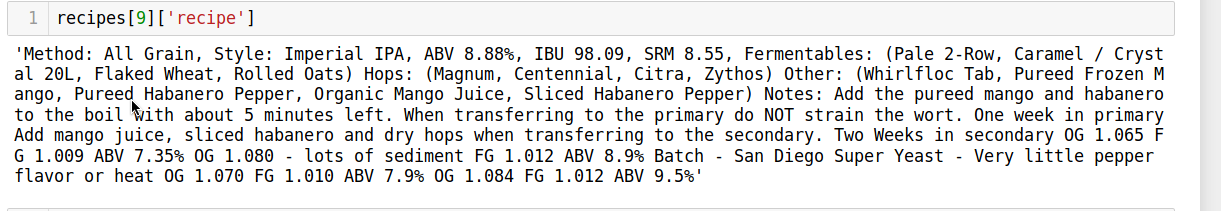
\includegraphics[height=0.2\textwidth]{beer_extraction.png}
    \caption{\label{beer_extraction}Example of self-extracted beer data} 
 \end{figure}
 As stated, some of the data that was extracted was identical to 
 that which came in the original dataset. 
 The additional data (see Figure \ref{beer_extraction}) here often contained the author Username, 
 fermentable ingredients, Steeping grains, Hops selection, 
 additional ingredients, and notes from the author. 
 This format was suitable for Elasticsearch full text queries, 
 but it was limited in its use for further data analysis outside of 
 aggregation counts of terms that occurred in the data.

 \subsubsection{Data Processing}
 \begin{figure}
    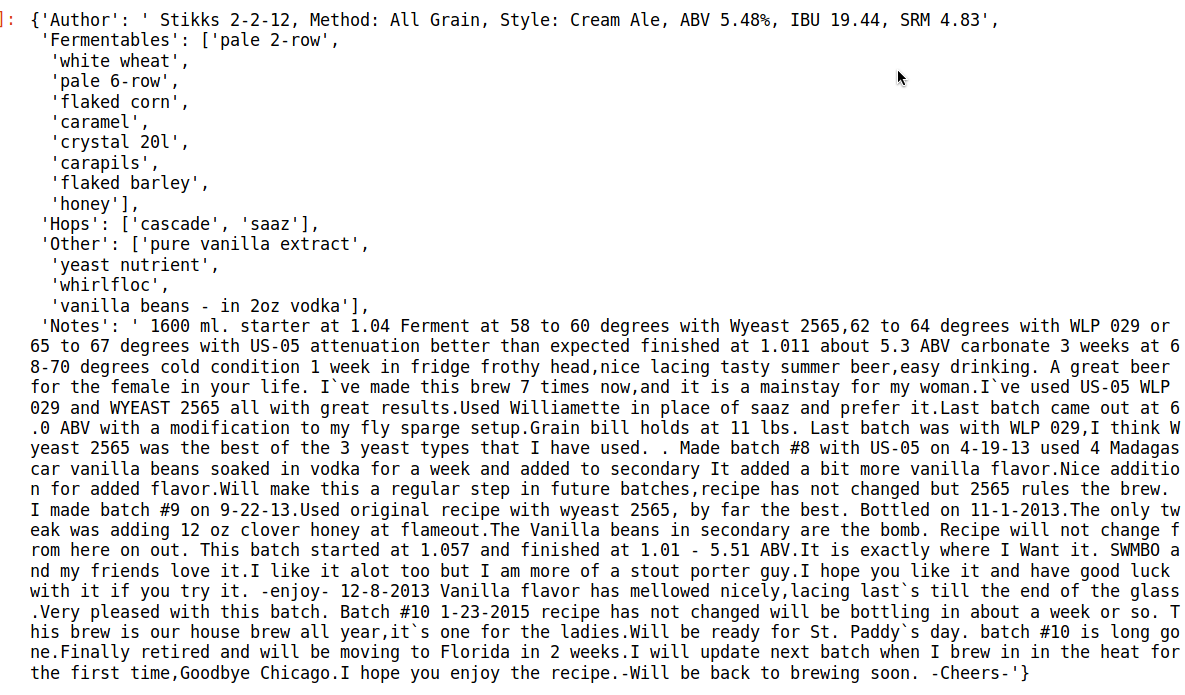
\includegraphics[height=0.5\textwidth]{beer_data_processing.png}
    \caption{\label{beer_data_processing} Example of a beer datapoint } 
 \end{figure}
 Beyond extraction, there was a significant amount of cleaning and 
 preprocessing that need to be done to make it more usable for 
 analysis (see Figure \ref{beer_data_processing}). From the sing string that was extracted, there were several 
 aspects that should have been extracted, such as ingredients and 
 notes. There were four different categories of ingredients to 
 extract and in addition, much of the data contained typos and 
 short hand for different ingredients and descriptions in the notes. 
 Much further refinements would also be necessary to make the data 
 more presentable. 

\subsection{Kibana}
\begin{figure}
   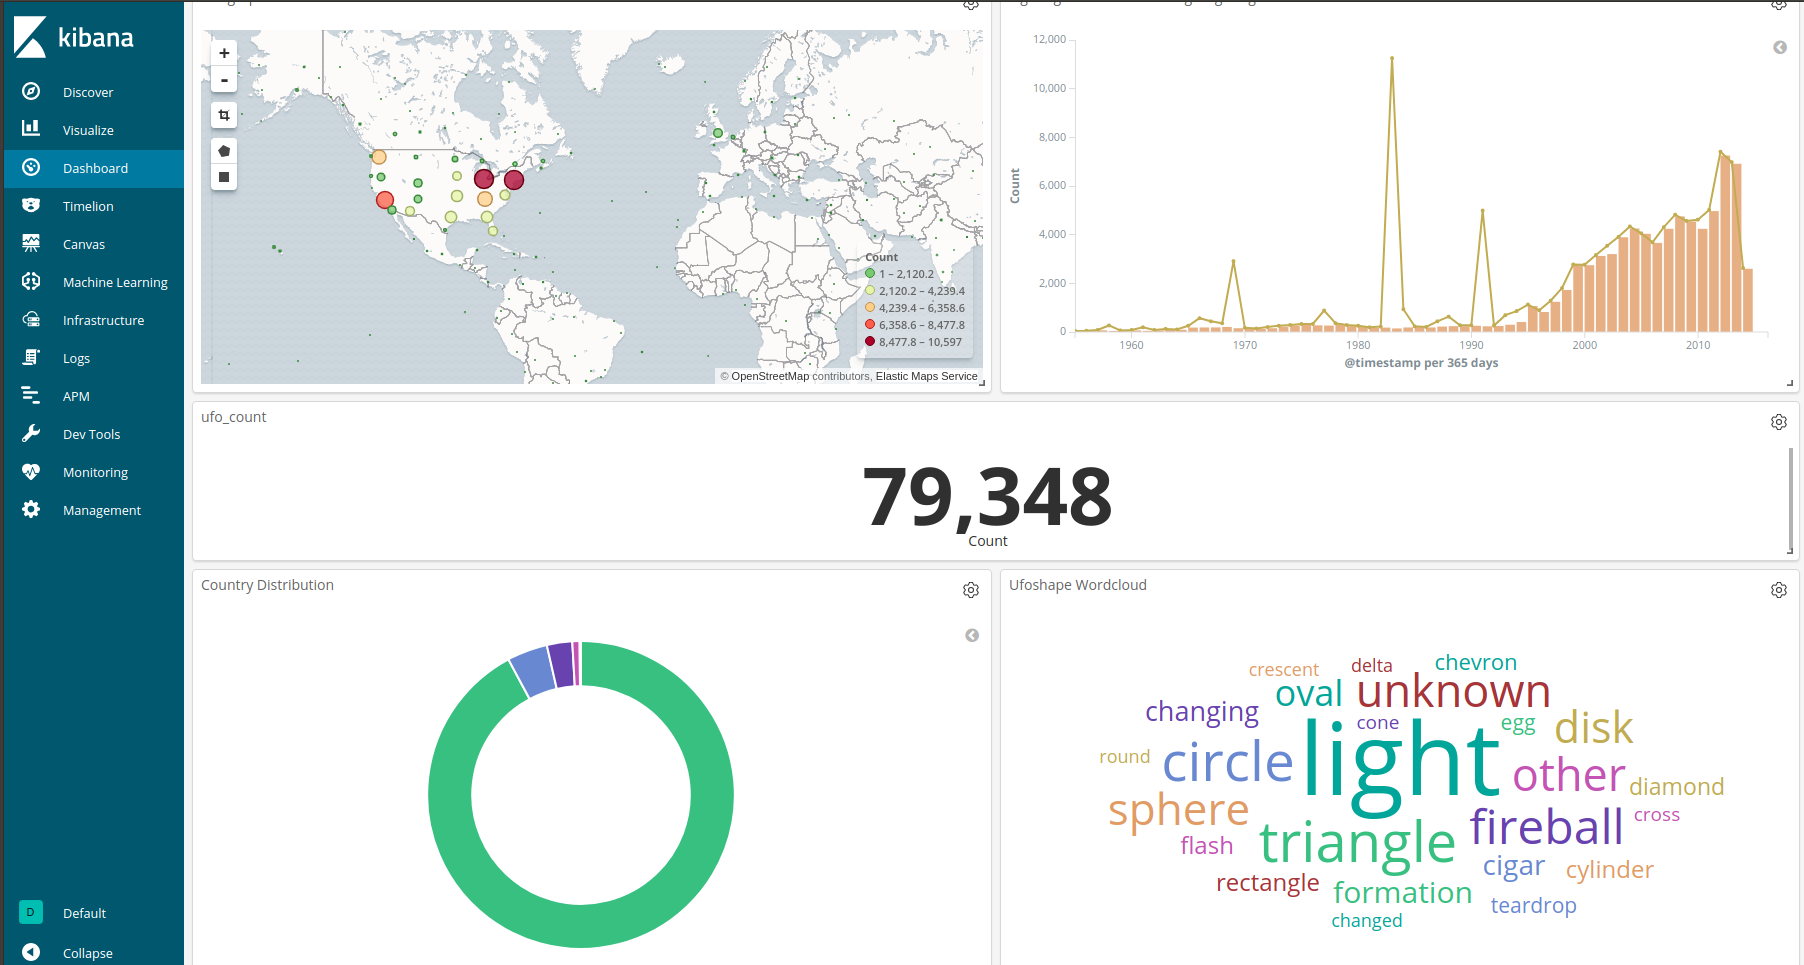
\includegraphics[height=0.5\textwidth]{dashboard1.png} 
   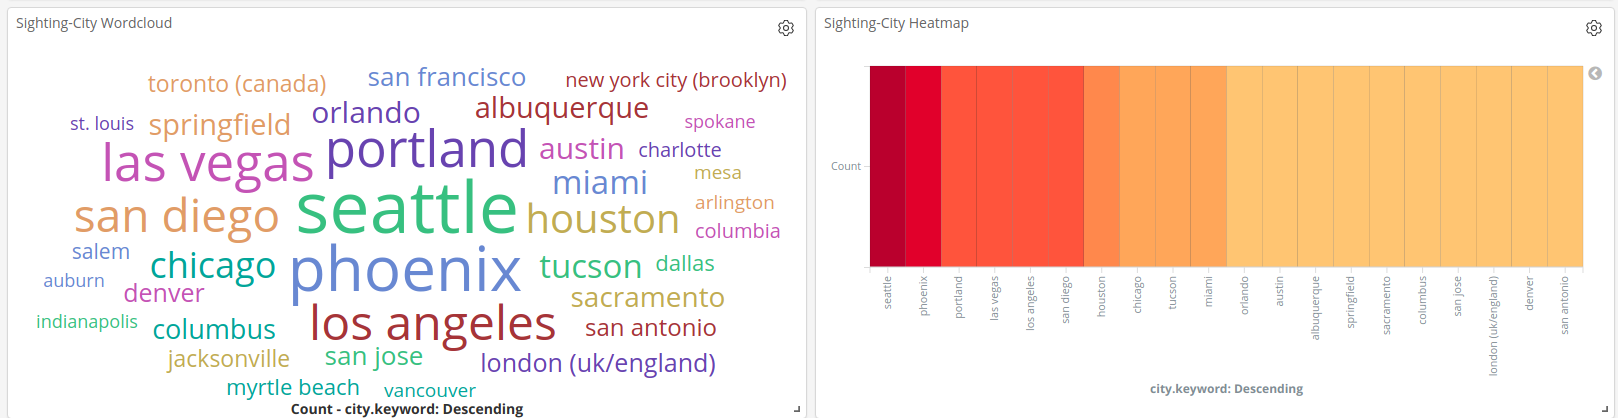
\includegraphics[height=0.242\textwidth]{dashboard2.png} 
   \caption{\label{ufo_dashboard}The dashboard for the Ufo-dataset}
\end{figure}
\begin{figure}
   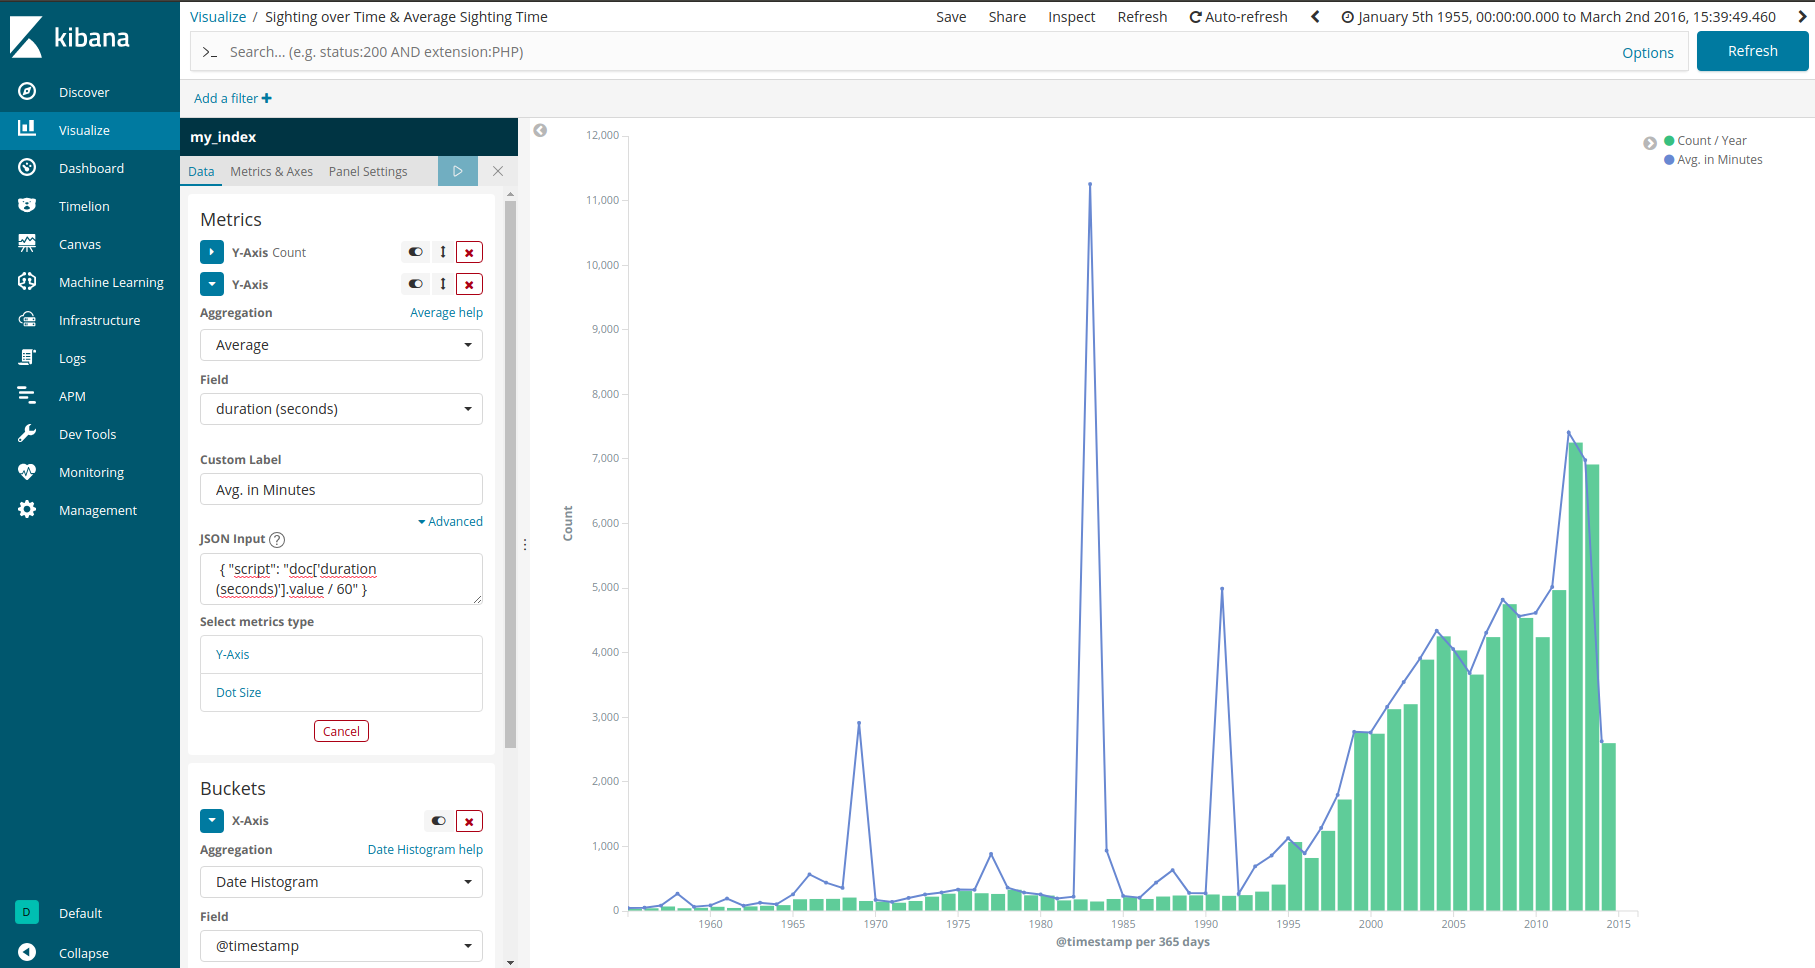
\includegraphics[height=0.5\textwidth]{kibana_script.png} 
   \caption{\label{json_script}This is an visualization in the editive mode.}
\end{figure}
In the previous Section the speed, flexibility and powerfull search capability
were shown. But technical power alone is rarely enough. In order to work with data 
one has to have a good intuition about it. And since the human brain is better in 
interpreting images than a matrix of values a common approach for better understanding data 
is to visualize it.
\\
Kibana is a simple to use and still powerfull visualization tool which it build on top 
of Elasticsearch. It comes with a lot of inbuild visualizations: Histograms, 
Pie Charts, Lines, Heat Maps, Geographical Maps etc. These visualizations can be organized
in dashboards. The dashboards are interactive, which means if one clicks on 
a value in a visualization (e.g. the biggest part in a Pie Chart) this value is used
as a filter for all visualizations which are part of the same dashboard.
This functionality makes explorative descriptive statistics really convinient, 
because different aspects of the data can be looked at by playing and clicking
around in the dashboard.
\\
Additionally Kibana provides a lot more functionalities like Machine Learning
based anomaly detection, customizable visualizations which are not in the scope of this report.
\\
But one additional functionality has to be mentioned at this point. It is the 
possibility to create online scripts, which process data on the fly. In Figure \ref{json_script} 
the \textit{JSON Input} field is an example for such a script. This script turns seconds
into minutes by dividing the current value by 60. That way the original data does not
need to be touched and the calculation is done only for the visualization. The drawback of this
scripting functionality is, that the script needs to be run every time the visualization is loaded.
For huge datasets this can lead to long waiting times, especially when the scripting 
functionality is used in many visualizations.
\\
\\
In Figure \ref{ufo_dashboard} different visualizations are shown for the ufo dataset,
which are organized into a dashboard:
\\
In the upper left, a geographical visualization is shown. It marks all the points
where ufos were seen. Bigger circles are collections of datapoints. This can be seen
by zooming in, then the bigger circle is devided into multiple smaller circles.
\\
In the upper right a histogram and a line is shown. The histogram describes
how many ufo sightings were recorded per year. The line is the average time 
(in minutes) per year that ufo's were seen\footnote{The line is not on the same scale as the histogram.
In order to see the actual minutes-values one needs to hover with the mouse to the point of interest.}.
Since the line visualization contains an outlier around 1964, this would
be a typical scenario to apply a filter by clicking on the outlier and inspecting the results of the other visualizations. That way
it could be investigated if something interesting happened in 1964 or if this was
an error during data collection.
\\
The next visualization below is just a simple count of data points (size of the dataset). 
In a live application this would be more interesting, because one could inspect how the 
dataset grows.
\\
Below that on the left there is a Pie Chart which shows the distribution over Countries:
Green = America, Blue = Canada, Violett = Great Britain, Purple = Australia, Red = Germany (not visible anymore on the PDF).
\\
On the right of the Pie Chart there is a frequency based wordcloud, showing the different ufo shapes which 
people described during the ufo sighting. It has to be mentioned that it is only possible to
use a wordloud properly on (pseudo) categorical values - only one word per field. There is not preprocessing step
(like tokenization) involved.
\\
Below on the left is again a wordcloud which shows roughly the distribution over cities.
\\
To the right of the city wordcloud, the information about cities is encoded as a 
heatmap (just for the sake of showing exploring different visualizations).
\\
\\
As a quick summary and interpretation of the visualization the following can 
be recorded: most of the ufo sightings happened in the US; in 1964 there might have been 
an ufo boom; lights, circles, triangles, fireballs are popular descriptions of the ufo-look;
seattle, phoenix, portland, las vegas are the most popular cities were people claim to have seen ufos.


\begin{figure}
  \centering
  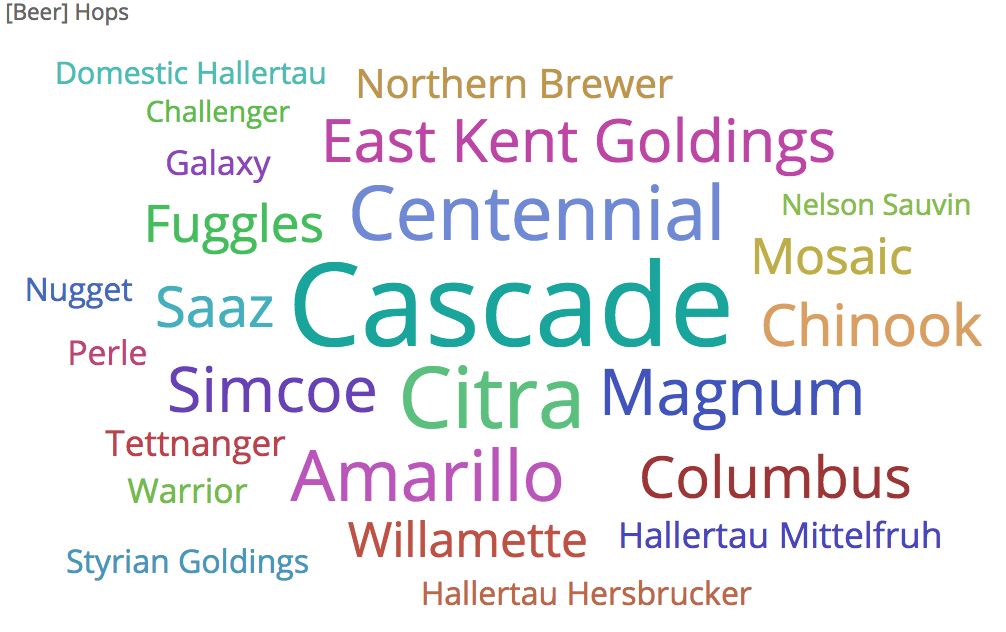
\includegraphics[width=\linewidth]{beer_hops.png}
 \caption{Word cloud for ``hops'' field for the whole dataset on Kibana Dashboard}
  \label{fig:beer_hops}
\end{figure}


Another useful feature is 'control' in Kibana dashboard. It is essentially a filter function to visualise a subset of the dataset. It is a useful interactive tool to investigate the relationships between different fields in the dataset.



\begin{figure}
  \centering
  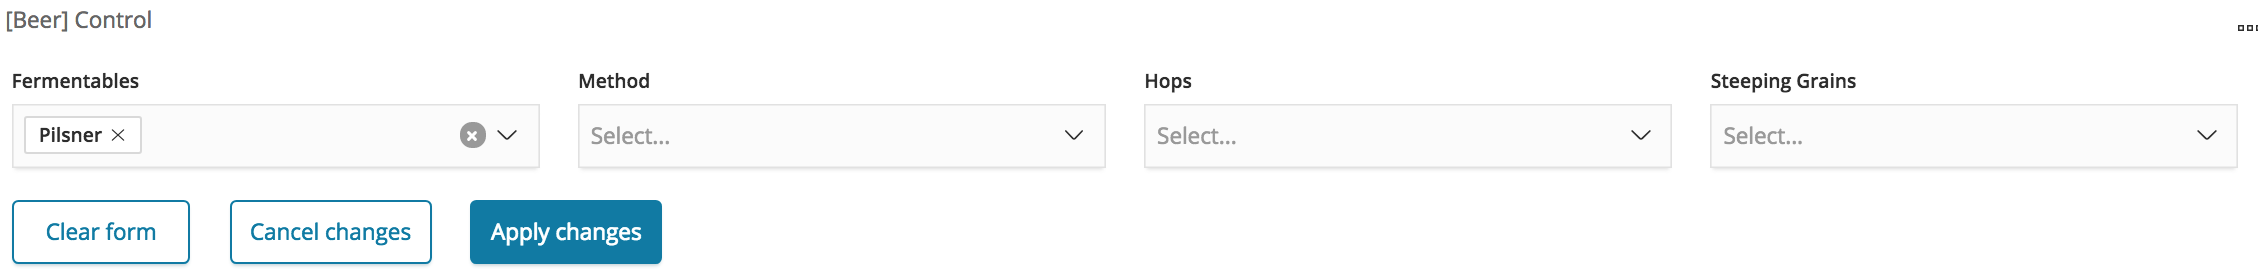
\includegraphics[width=\linewidth]{beer_control.png}
 \caption{Example control on Kibana Dashboard}
  \label{fig:beer_control}
\end{figure}

For example, the most common hops in whole beer recipe dataset is ``cascade''. (see Figure \ref{fig:beer_hops}) After selecting the ``Pilsner'' in the ``Fermentable'' filter (Figure \ref{fig:beer_control}), the distribution of the resulting dataset is altered, showing that the most common hops for ``Pilsner'' is ``saaz'', instead of ``cascade'' (Figure \ref{fig:beer_hops_after}). 

\begin{figure}
  \centering
  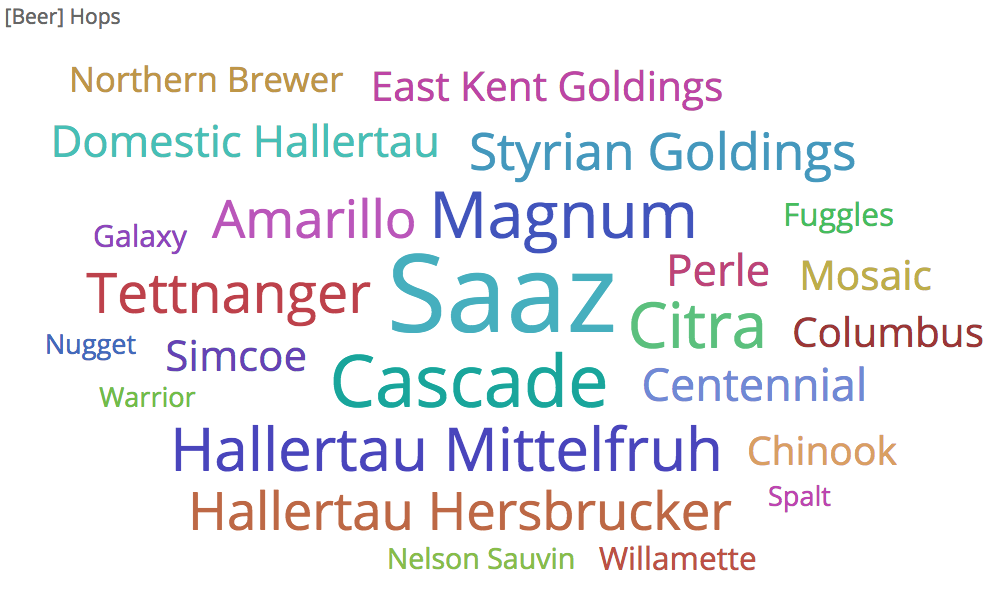
\includegraphics[width=\linewidth]{beer_hops_after.png}
 \caption{Hops distribution changed after a filter is applied}
  \label{fig:beer_hops_after}
\end{figure}



\section{Conclusion}
Fast, Powerfull bla bla bla...

\section{Personal Reflection}
Here we can put our personal opinions and say what we liked most.

\end{document}